\documentclass[twocolumn]{article}

% Use Unicode by default for using special characters
\usepackage[utf8]{inputenc}
% Mathematical Symbols and fonts
\usepackage{amsmath}
% For inserting figures
\usepackage{graphicx}
% To insert URLs on which you can click
\usepackage{url}
% Bibliography citations
\usepackage[round]{natbib}
% To make two column figures appear in the correct order
\usepackage{fixltx2e}
% To make annotations on the sides
\usepackage{todonotes}
% To generate dummy text
\usepackage{lipsum}

% Document metadata
%%%%%%%%%%%%%%%%%%%%%%%%%%%%%%%%%%%%%%%%%%%%%%%%%%%%%%%%%%%%%%%%%%%%%%%%%%%%%%%
\newcommand{\Title}{
    {{ cookiecutter.title }}
}
\newcommand{\Keywords}{
    Inverse theory;
    Gravity anomalies and Earth structure;
    Satellite gravity;
    South America;
}
\title{\Title}
\author{ 
    {{ name }}, 
}
% Metadata for the generated PDF
\usepackage[pdftex,colorlinks=true]{hyperref}
\hypersetup{
    pdftitle={\Title},
    pdfauthor={ {{ name }},  },
    pdfkeywords={\Keywords},
    pdfcreator={pdfTeX},
    allcolors=black,
}


%%%%%%%%%%%%%%%%%%%%%%%%%%%%%%%%%%%%%%%%%%%%%%%%%%%%%%%%%%%%%%%%%%%%%%%%%%%%%%%
\begin{document}

    \maketitle

    \begin{abstract}
        \lipsum[1]
    \end{abstract}

    \section{Introduction}

Cite things using \citet{tikhonov1977} or \citep{tikhonov1977}.

\lipsum[2]

    \section{Methodology}

\lipsum[3]

\subsection{Software implementation}

Describe the implementation, where the code is located (Github and
figshare/zenodo), and the license.
Cite the dependencies that we are using:
scipy and numpy \citep{numpy},
matplotlib \citep{matplotlib},
Fatiando a Terra \citep{fatiando},
Jupyter notebook\citep{jupyter}.

    \section{Results}

\lipsum[5]

\begin{figure}
    \centering
    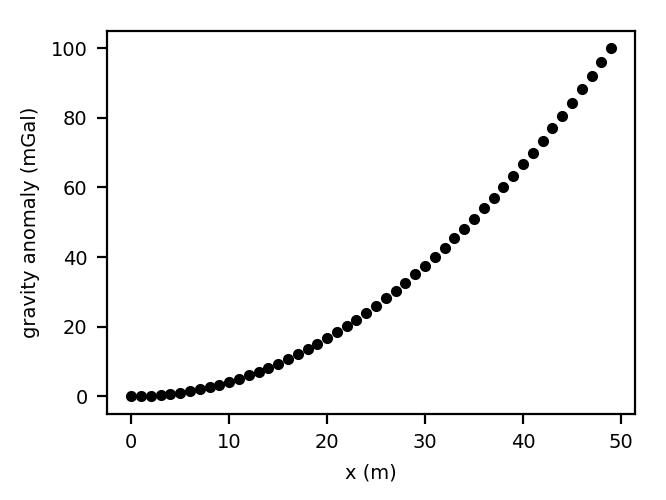
\includegraphics[]{../figures/summary}
    \caption{
        Example image.
    }
    \label{fig:meh}
\end{figure}

    \section{Discussion}

\lipsum[7]

    \section{Conclusions}

\lipsum[9]


    \section{Acknowledgments}

    We are indebted to the developers and maintainers of the open-source
    software without which this work would not have been possible.
    \textbf{Thank reviewers, editors, and funding agencies.}

    \bibliographystyle{plainnat}
    \bibliography{references}

\end{document}
